\documentclass[
    11pt, % Set the default font size, options include: 8pt, 9pt, 10pt, 11pt, 12pt, 14pt, 17pt, 20pt
    %
    aspectratio=169, % Uncomment to set the aspect ratio to a 16:9 ratio which matches the aspect ratio of 1080p and 4K screens and projectors
]{beamer}
\usepackage{hyperref}
%\graphicspath{{Images/}{./}} % Specifies where to look for included images (trailing slash required)
\usepackage{booktabs} % Allows the use of \toprule, \midrule and \bottomrule for better rules in tables

%\usepackage{appendixnumberbeamer} %If you want a separate slide counter for your appendix

%%% Customize Theme %%%%%%%%%%%%%%%%%%%%%%
\usetheme{Madrid} % You can use other themes too, but this changes many things. I've found Madrid to be the best for this color scheme

%fg = font color
%bg = background color

% ! WARNING ! : Many colors are linked to multiple attributes, so changing one color can have unexpected changes!

% If you want to tweak the shading of orange and red, tweak the below 2 lines:t
\definecolor{myRed}{RGB}{120,4,4}
\definecolor{myOrange}{RGB}{227, 125, 0}

% Bottom right hand color
\setbeamercolor*{structure}{bg=myRed!20,fg=myRed!90}

\setbeamercolor*{palette primary}{use=structure,fg=white,bg=structure.fg} %?
\setbeamercolor*{palette secondary}{use=structure,fg=myRed,bg=white}
    %bottom left of footer & bar between title & top bubbles
\setbeamercolor*{palette tertiary}{use=structure,fg=white,bg=myRed} 

\setbeamercolor{frametitle}{bg=myRed!85,fg=white} %title of each slide

\setbeamercolor*{titlelike}{parent=palette primary} %?
%\setbeamercolor{titlelike}{parent=palette primary,fg=structure.fg!50!myRed}

%for miniframe (very top) AND center footer
\setbeamercolor{section in head/foot}{fg=myOrange, bg=white}

%%% Specific Colors %%%
\setbeamercolor{item projected}{bg=myOrange}
\setbeamertemplate{enumerate items}{bg=myOrange}

\setbeamercolor{itemize item}{fg=myOrange}
\setbeamercolor{itemize subitem}{fg=myOrange}

\setbeamercolor{button}{bg=myOrange}

%%% Edits ONLY the TOC slide %%%
\setbeamercolor{section in toc}{fg=black}
\setbeamercolor{subsection in toc}{fg=black}

%%% Block Colors %%%
% Standard block %
    \setbeamercolor{block title}{bg=myOrange, fg=white}
    \setbeamercolor{block body}{bg=myOrange!20}

% Alerted block % If you want to customize it's color
    %\setbeamercolor{block title alerted}{bg=cyan, fg=white}
    %\setbeamercolor{block body alerted}{bg=cyan!10}

% Example block % If you want to customize it's color
    %\setbeamercolor{block title example}{bg=cyan, fg=white}
    %\setbeamercolor{block body example}{bg=cyan!10}

%---------------------------------------------------------
%	SELECT FONT THEME & FONTS
%---------------------------------------------------------
\usefonttheme{default} % Typeset using the default sans serif font
\usepackage{palatino} % Use the Palatino font for serif text
\usepackage[default]{opensans} % Use the Open Sans font for sans serif text
\useinnertheme{circles}

%---------------------------------------------------------
%	SELECT OUTER THEME
%---------------------------------------------------------
% Outer themes change the overall layout of slides, such as: header and footer lines, sidebars and slide titles. Uncomment each theme in turn to see what changes it makes to your presentation.

%\useoutertheme{default}
%
\useoutertheme{miniframes}

%\useoutertheme{infolines}
%\useoutertheme{smoothbars}
%\useoutertheme{sidebar}
%\useoutertheme{split}
%\useoutertheme{shadow}
%\useoutertheme{tree}
%\useoutertheme{smoothtree}

%---------------------------------------------------------
%	PRESENTATION INFORMATION
%---------------------------------------------------------

\title[Paleocomplexity]{Quantum Computing Since Democritus}
\subtitle{Scott Aaronson}
\author[Quantum Computing Since Democritus]{Chapter 5: Paleocomplexity}

\institute[]{Saumya Chaturvedi \\ \smallskip }
\date[27 March 2023]
%\date[\today]


%---------------------------------------------------------
%---------------------------------------------------------
%---------------------------------------------------------
\begin{document}

%---------------------------------------------------------
%	TITLE SLIDE
%---------------------------------------------------------
\section{}
\begin{frame}
	\titlepage % Output the title slide, automatically created using the text entered in the PRESENTATION INFORMATION block above
 
\end{frame}

%---------------------------------------------------------
%	TABLE OF CONTENTS SLIDE
%---------------------------------------------------------

\begin{frame}
	\frametitle{Table of Contents} % Slide title, remove this command for no title
	
	\tableofcontents % Output the table of contents (all sections on one slide)
	%\tableofcontents[pausesections] % Output the table of contents (break sections up across separate slides)
\end{frame}

%---------------------------------------------------------
%	PRESENTATION BODY SLIDES
\section{Eras}
\begin{frame}{Glory of Computability Theory}
    \begin{itemize}
        \item Mankind's greatest victories: fire, wheel, computability theory.
        \item To understand how quantum mechanics changed things, need to examine scene before it.
        \item Divide complexity history into chapters: 
        
        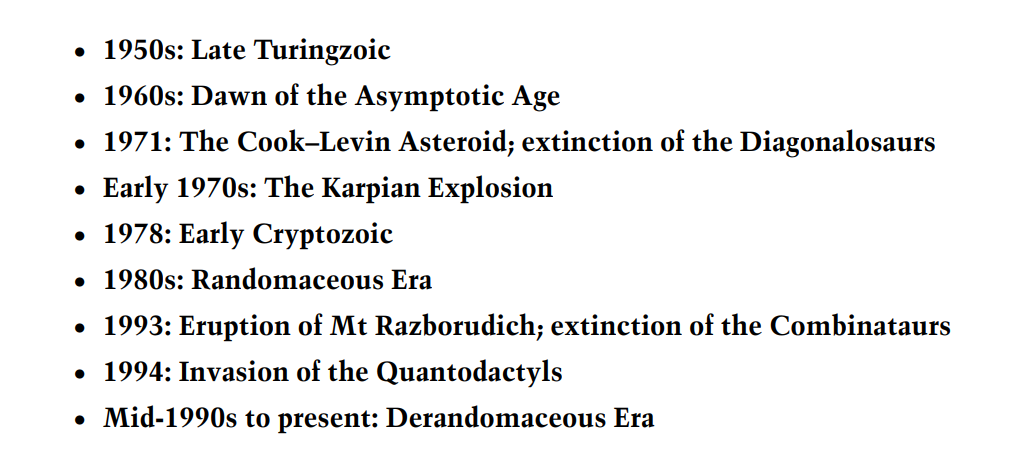
\includegraphics[angle=0,width=10cm,height=3.5cm]{complexityeras.png}
    \end{itemize}
\end{frame}

\begin{frame}{Paleocomplexity}
\begin{itemize}
    \item Complexity in the era before P, NP, when Diagonalosaurs ruled. 
    \item Uncomputable problems about positive integers.
    \item But say I give you: For all real x and y, $(x + y)^2 = x^2 + 2xy + y^2$
    \item Tarski Decision Procedure: algorithm for deciding on the validity of any elementary statement about polynomials over the field of real numbers. 
    \item Bonus: Complex analysis to encode Godel statements (can force n in $e^{2in\pi}$ to be anything).
\end{itemize}
\end{frame}

\section{Decision Procedure}
\begin{frame}{Problem Solved? No.}
    \begin{itemize}
        \item Deciding truth of a sentence with n symbols, it grows like \def\rddots#1{\cdot^{\cdot^{\cdot^{#1}}}}
$ 2^{2^{\rddots2}} $
\bye (n times).
        \item On the computers of 1950s, it was \def\rddots#1{\cdot^{\cdot^{\cdot^{#1}}}}
$ hopeless^{hopeless^{\rddots...}} $
    \end{itemize}
\end{frame}

\section{Complexity}
\begin{frame}{What is complexity?}
    \begin{itemize}
        \item Putting an upper bound on resources your computer can use.
        \item Obvious ones:
        \begin{itemize}
            \item Amount of time
            \item Amount of memory
        \end{itemize}
        \item But 500s others too! 
        \item Different from Computer Architecture (How much can be computed in 10 million steps/bits?)
        \item Rephrase: How much in an amount of time that grows linearly?
    \end{itemize}
\end{frame}

\section{Time and Space}
\begin{frame}{Time and Space}
\begin{itemize}
    \item TIME$(f(n))$: class of problems for which every instance of size n is solvable in amount of time that grows like a constant $* f(n)$.
    \item "solvable": by an idealised computer (eg., Turing Machine), fixed as "reference".
    \item Not much dependent on the reference when under broad limits (like classical computers only).
    \item<1-> SPACE$(f(n))$: class of problems solvable by reference machine using amount of space (i.e., bits of memory) that grows like a constant $* f(n)$.
    \item<2-> TIME$(f(n))$ contained in SPACE$(f(n))$ (can access only 1 memory location per step).
\end{itemize}
\end{frame}

\section{Time Hierarchy Theorem}
\begin{frame}{Time Hierarchy Theorem}
    \begin{itemize}
        \item TIME$(n^2)$ contained in TIME$(n^3)$. 
        \item<1-> Strictly contained?
        \item<2-> Can we solve more problems in $n^3$ time than in $n^2$ time?
        \item<3-> Time Hierarchy Theorem got Hartmanis and Stearns a Turing Award in the mid-1960s.
        \item<3-> Analogous: Space Hierarchy Theorem.
    \end{itemize}
\end{frame}

\begin{frame}{Proof}
    \begin{itemize}
        \item A time-bounded analog of Turing’s halting problem!
        \item \textit{Given a Turing machine M, does M halt in at most $n^{2.5}$ steps?}
        \item Clearly solvable in $n^{2.5}$ log $n$ steps.
        \item To prove unsolvable in $n^2$ steps, check proof by Contradiction on whiteboard.
    \end{itemize}
\end{frame}

\section{Time-Constructibility}
\begin{frame}{Time-Constructibility}
    \begin{itemize}
        \item<1-> Substitute any functions $f$ and $g$ such that $f$ grows significantly faster than $g$?
        \item<2-> No! $g$ needs to be time-constructible.
        \item There's some program that halts in $g(n)$ steps given $n$ as input.
        \item Making growing functions that weren't time-constructible. (function $f(n)$ such that TIME$f(n)$ = TIME$2^{f(n)}$).
    \end{itemize}
\end{frame}

\section{Blum Speedup Theorem}
\begin{frame}{Fastest Algorithm}
    \begin{itemize}
        \item Is there always a fastest algorithm?
        \item Multipying 2 n-by-n matrices.
        \item Obvious answer: $O(n^3)$ time. But fastest time is $O(n^{2.373})$ in 2011. 
        \item Could we make it closer to $O(n^2)$, but have the algorithms become endlessly complicated?
    \end{itemize}
\end{frame}

\begin{frame}{What if there isn't one?}
    \begin{itemize}
        \item Infinite sequence of algorithms, each faster than the last, but slower than some algorithm.
        \item Blum Speedup Theorem in 1967, kindof obsolete now.
        \item There exists a problem P s.t., for every function $f$, if P has an $O(f(n))$ algorithm then it also has an $O(log f(n))$ algorithm!
        \item For any complexity measure, there exists a computable function, such that there is no optimal program computing it, because every program has a program of lower complexity. 
        \item Godel Speed-up Theorem: shortening proofs by working in more powerful axiomatic systems. 
    \end{itemize}
\end{frame}

\section{Solution to Puzzles!}
\begin{frame}{Solution to Puzzles!}
\centering
    Check out the book!
\end{frame}


\end{document}
